% Comentarios para Plos {{{
% The manuscript LaTeX source should be contained within a single file (do not use \input, \externaldocument, or similar commands).
%
% -- FIGURES AND TABLES
%
% Please include tables/figure captions directly after the paragraph where they are first cited in the text.
%
% DO NOT INCLUDE GRAPHICS IN YOUR MANUSCRIPT
% - Figures should be uploaded separately from your manuscript file. 
% - Figures generated using LaTeX should be extracted and removed from the PDF before submission. 
% - Figures containing multiple panels/subfigures must be combined into one image file before submission.
% For figure citations, please use "Fig" instead of "Figure".
% See http://journals.plos.org/plosone/s/figures for PLOS figure guidelines.
%
% Tables should be cell-based and may not contain:
% - spacing/line breaks within cells to alter layout or alignment
% - do not nest tabular environments (no tabular environments within tabular environments)
% - no graphics or colored text (cell background color/shading OK)
% See http://journals.plos.org/plosone/s/tables for table guidelines.
%
% For tables that exceed the width of the text column, use the adjustwidth environment as illustrated in the example table in text below.
%
% % % % % % % % % % % % % % % % % % % % % % % %
%
% -- EQUATIONS, MATH SYMBOLS, SUBSCRIPTS, AND SUPERSCRIPTS
%
% IMPORTANT
% Below are a few tips to help format your equations and other special characters according to our specifications. For more tips to help reduce the possibility of formatting errors during conversion, please see our LaTeX guidelines at http://journals.plos.org/plosone/s/latex
%
% When adding superscript or subscripts outside of brackets/braces, please group using {}.  For example, change "[U(D,E,\gamma)]^2" to "{[U(D,E,\gamma)]}^2". 
%
% Do not use \cal for caligraphic font.  Instead, use \mathcal{}
% }}}

\documentclass[10pt,letterpaper]{article} % {{{
\usepackage[top=0.85in,left=2.75in,footskip=0.75in]{geometry}

\usepackage{amsmath,amssymb}
\usepackage{changepage}
\usepackage[utf8x]{inputenc}
% \usepackage{textcomp,marvosym}
\usepackage{cite}
% Use nameref to cite supporting information files (see Supporting Information section for more info)
\usepackage{nameref,hyperref}
\usepackage[right]{lineno}

% ligatures disabled
\usepackage{microtype}
\DisableLigatures[f]{encoding = *, family = * }

% color can be used to apply background shading to table cells only
\usepackage[table]{xcolor}
\usepackage{array}
\usepackage{caption}
\usepackage{multirow}
\usepackage{booktabs}
\usepackage{pdfpages}
\usepackage{tcolorbox}
\usepackage{colortbl}
\usepackage[draft,inline,nomargin]{fixme} \fxsetup{theme=color}
\FXRegisterAuthor{jm}{jmm}{\color{purple}Josue}
\FXRegisterAuthor{cp}{acp}{\color{blue}CP}
\FXRegisterAuthor{cg}{cgg}{\color{red}CG}
\definecolor{C1-EN}{RGB}{0,132,170}
\definecolor{C1-FR}{RGB}{255,117,0}
\definecolor{C1-GE}{RGB}{134,0,179}
\definecolor{C1-IT}{RGB}{49,129,6}
\definecolor{C1-SP}{RGB}{162,0,0}

\newcolumntype{+}{!{\vrule width 2pt}}

% create \thickcline for thick horizontal lines of variable length
\newlength\savedwidth
\newcommand\thickcline[1]{%
  \noalign{\global\savedwidth\arrayrulewidth\global\arrayrulewidth 2pt}%
  \cline{#1}%
  \noalign{\vskip\arrayrulewidth}%
  \noalign{\global\arrayrulewidth\savedwidth}%
}

% \thickhline command for thick horizontal lines that span the table
\newcommand\thickhline{\noalign{\global\savedwidth\arrayrulewidth\global\arrayrulewidth 2pt}%
\hline
\noalign{\global\arrayrulewidth\savedwidth}}


% Remove comment for double spacing
%\usepackage{setspace} 
%\doublespacing

% Text layout
\raggedright
\setlength{\parindent}{0.5cm}
\textwidth 5.25in 
\textheight 8.75in

% Bold the 'Figure #' in the caption and separate it from the title/caption with a period
% Captions will be left justified
\usepackage[aboveskip=1pt,labelfont=bf,labelsep=period,justification=raggedright,singlelinecheck=off]{caption}
\renewcommand{\figurename}{Fig}

% Use the PLoS provided BiBTeX style
\bibliographystyle{plos2015}

% Remove brackets from numbering in List of References
\makeatletter
\renewcommand{\@biblabel}[1]{\quad#1.}
\makeatother



% Header and Footer with logo
\usepackage{lastpage,fancyhdr,graphicx}
\usepackage{epstopdf}
%\pagestyle{myheadings}
\pagestyle{fancy}
\fancyhf{}
%\setlength{\headheight}{27.023pt}
%\lhead{\includegraphics[width=2.0in]{PLOS-submission.eps}}
\rfoot{\thepage/\pageref{LastPage}}
\renewcommand{\headrulewidth}{0pt}
\renewcommand{\footrule}{\hrule height 2pt \vspace{2mm}}
\fancyheadoffset[L]{2.25in}
\fancyfootoffset[L]{2.25in}
\lfoot{\today}

%% Include all macros below

\newcommand{\lorem}{{\bf LOREM}}
\newcommand{\ipsum}{{\bf IPSUM}}

%% END MACROS SECTION

% }}}
\begin{document}
% Autores, titulo y otros {{{
\vspace*{0.2in}

% Title must be 250 characters or less.
\begin{flushleft}
{\Large
\textbf\newline{Statistical analysis of 1-grams flow among Indo-European languages} % Please use "sentence case" for title and headings (capitalize only the first word in a title (or heading), the first word in a subtitle (or subheading), and any proper nouns).
}
\newline
% Insert author names, affiliations and corresponding author email (do not include titles, positions, or degrees).
% \\
% \cpnote{Discutir los autores: Josue, CarlosG, FLores, CarlosP, quizá sergio? Fernanda? } 

Josué Ely Molina  \ddag\textsuperscript{1,2}, %\textsuperscript{1,2\Yinyang},
Jorge Flores      \dag \textsuperscript{2}, %\textcurrency},
Carlos Gershenson \textsuperscript{3,4},
Sergio Sanchez    \textsuperscript{5},
Carlos Pineda     \ddag\textsuperscript{2,*}    % \textsuperscript{2\Yinyang},
%Name5 Surname \textsuperscript{2\ddag},
%Name6 Surname \textsuperscript{2\ddag},
%Name7 Surname \textsuperscript{1,2,3*},

%with the Lorem Ipsum Consortium\textsuperscript{\textpilcrow}

\newcommand{\unam}{Universidad Nacional Aut\'{o}noma de
M\'{e}xico, Mexico City, 01000, Mexico}
% \address[1]{Instituto de F\'{\i}sica, \unam}
% \address[2]{Centro de Ciencias de la Complejidad, \unam}
% \address[4]{ Instituto de Investigaciones en Matem\'{a}ticas Aplicadas y Sistemas, \unam }
% \address[6]{
% 
% }
% 

%\\
\bigskip
\textbf{1} Facultad de Ciencias, \unam \\
\textbf{2} Instituto de F\'{\i}sica, \unam \\
\textbf{3} Instituto de Investigaciones en Matem\'{a}ticas Aplicadas y Sistemas, \unam \\
\textbf{4} Centro de Ciencias de la Complejidad, \unam \\
\textbf{5} 
Maestr\'{\i}a en Ciencias de la Complejidad, 
Universidad Aut\'{o}noma de la Ciudad de M\'{e}xico,
Mexico City, Mexico
\\
\bigskip

% Insert additional author notes using the symbols described below. Insert symbol callouts after author names as necessary.
% 
% Remove or comment out the author notes below if they aren't used.
%
% Primary Equal Contribution Note
% \Yinyang These authors contributed equally to this work.

% Additional Equal Contribution Note
% Also use this double-dagger symbol for special authorship notes, such as senior authorship.
\ddag These authors also contributed equally to this work.

% Current address notes
% \textcurrency Current Address: Dept/Program/Center, Institution Name, City, State, Country % change symbol to "\textcurrency a" if more than one current address note
% \textcurrency b Insert second current address 
% \textcurrency c Insert third current address

% Deceased author note
\dag Deceased

% Group/Consortium Author Note
% \textpilcrow Membership list can be found in the Acknowledgments section.

% Use the asterisk to denote corresponding authorship and provide email address in note below.
* carlospgmat03@gmail.com

\end{flushleft}
% Please keep the abstract below 300 words
% }}}
\section*{Abstract} % {{{
\cpnote{Por hacer al final}
% }}}

\linenumbers
% Use "Eq" instead of "Equation" for equation citations.
% For figure citations, please use "Fig" instead of "Figure".
\section*{Introduction} % {{{

% \cpnote{No me gusta el inicio de la intro. Como que sugiere que hacemos el 
% estudio porque podemos. Creo qe toca pensar mejor la justificacion y abrir 
% en esa direccion. Me gusta mucho mas el segundo parrafo y quizá quisiera iniciar
% de esa manera.}
% \jmnote{Modifique el primer parrafo, el parrafo viejo quedo en el text comentado}

\cpnote{Aun no hay una justiicación de por que estudiamos lo que estudiamos. Si quieres
lo platicamos con CarlosG la siguiente vez que nos veamos. Mientras piensa un poco y 
si quieres platicar conmigo, lo podemos hacer.}
In recent years, the emergence and development of computational tools has
benefited various statistical studies to understand certain characteristics of
the human population. For example, we are able to predict the growth rate of a
city, the number of people who have watched a movie, the user traffic on a web
page, and even the way we use words in written language. The previous examples
are cases of the Zipf's law, formulated by George Zipf in 1940~\cite{Zipf} upon
discovering that if  the words used in a text are ranked by their frequency of
appearance, where the lower ranks belong to the most frequent words,  then the
frequency  $f$  of any word and its rank  $k$ are related by a power law of the
form $f~1/k$.



 
%In recent years, the field of linguistics has been benefited from the
%development of more sophisticated computational tools, helping to process a
%greater amount of data in less time and allowing the study of linguistics
%from a statistical perspective.  This statistical study began with the works
%of George Zipf~\cite{Zipf}, in them Zipf argues that if  the words used in a
%text are ranked by their frequency of appearance,  where the lower ranks
%belong to the most frequent words,  then the frequency  f  of any word and its
%rank  k are related by a power law of the form f~1/k. The previous expression
%is known as  Zipf’s law, and it has not only been tested on language datasets,
%Morales et al.~\cite{Morales_epj} have also proved on sports and games data,
%and Cristelli et al.~\cite{Cristelli_zipfgdp} on the gross domestic product of
%several countries,  wealth of American citizens,  and population of cities.
 
Zipf's law has been mostly used to study the structures of language,
nonetheless, not enough studies have been done to understand the historical and
cultural features that language provides. One way to begin such a study is by
noting that the languages themselves are mixed, since within the vocabulary of
a language, from other languages are continuously added.
 
% %Although Zip’s law has opened several statistical studies in linguistics, nowadays few studies have been done about how within the vocabulary of a language, words from the language itself and from other languages are mixed
% \cpnote{Creo que podemos aca hablar mas de un mixing de cultura. Irnos de cosas generales a cosas particulares. Ahora, gracias a google ngram podemos aproximarnos a este problema mediante el lengauje}.
% \jmnote{modifique un poco este parrafo,  considero que el mixing del lneguaje y la cultura esta tratado en los sig parrafos}

Currently in the Spanish language, there are words from English 
that do not have a translation or that sometimes displace those that already
exist in Spanish.  For example, for native Spanish speakers it is common to
hear the word \textit{marketing} instead of its translation \textit{mercadeo}
when dealing with economic or business issues; also the word \textit{online}
has replaced \textit{en línea}, when referring to issues related to the
internet, a word officially adopted in Spanish.
 
This trending has not only affected Spanish,  but also other languages that are
being influenced by topics where English is the main and common language for
communication. However, in different periods of time, the flow of words came
from other languages. D’Amore~\cite{Damore_influencia_mutua} discusses with linguistic rigor the
flow of words between English and Spanish,  showing historical  and cultural
causes that allowed such flow; in addition to mentioning the influence of
Arabic in Spanish and French in English. \cpnote{Hay mas referencias, o es un 
caso singular?}
 
In this work, we use the Google Books N-gram~\cite{ngramv} dataset of the most
frequent words in books published in  English, French, German, Italian and
Spanish languages.  With that dataset,  we develop an algorithm that identifies
the words of one language  and that are being used exactly with the same 
spelling by others. Once these words
have been classified, we construct two models to quantify  the influence that
one language has had on another during the 20th century. The first model, we
count the number of new words that a language received from another, while in
the second method, we develop the concept of the use of one language in
another,  from quantifying the relative frequency of  the words of a language
that are being used in another language. In both we identify historical, social
and cultural causes that are responsible for the flow of words.
 
Next, we use the concept of rank diversity,  that shows the number of words
occupying a certain rank across the time. This study shows that  regardless of
who is the language the flow comes from or who language receives them,  the
lower ranks are always occupied by fewer  words, and as the rank increases the
diversity curve also increases as a logarithmic. 
 
\cpnote{Obvio aca toca poner algunos caveats y discutir la seccion de la estabilidad}

%\begin{eqnarray}
%\label{eq:schemeP}
%	\mathrm{P_Y} = \underbrace{H(Y_n) - H(Y_n|\mathbf{V}^{Y}_{n})}_{S_Y} + \underbrace{H(Y_n|\mathbf{V}^{Y}_{n})- H(Y_n|\mathbf{V}^{X,Y}_{n})}_{T_{X\rightarrow Y}},
%\end{eqnarray}
% }}}
\section*{Metodology} % {{{


For the development of this work,  we used the Google Books Ngram data set.
This dataset is made up of listing for each year and for each language of
publication the most used ``$n$-grams'' in the books of Google Books. 

The ``$n$-grams'' are the words or set of words that make up the text of a
book, where the number $n$ indicates the number of words that make up the gram,
being a 1-gram an individual word, a 2-gram a phrase composed of two 1-gram,
3-gram the set of three 1-gram and so on.

From this data set, the lists of the five thousand most used 1-grams each year
between 1740 and 2009 were extracted for the English, French, German, Italian
and Spanish languages. In each list, the words are ranked according to their
frequency of appearance, where the most frequent words have the lowest ranks.

\cpnote{Creo qe se tienen que unir los parrafos y decir de done salen esaos
ngrams, que son de libros escaneados}

To determine the presence of one language in another, an algorithm was
developed to find the words that are common between at least two languages,
these must be the same in writing, letter by letter. These words were defined as \textbf{migrant words}. \cpnote{Normalmente las palabras claves las pongo en italica. toca ver como le hace en el journal que elijamos.}

A migrant word is associated with a \textbf{source language} and a
\textbf{receiving language}, where the source language is the one where the
word appeared for the first time within the most used words,
while the receiving language is the one where the word is also present, being a
different set from the source language. In both sets, we are considering the five thousand most used words, since all the lists of the six languages (between 1740 and 2009), have at least this amount.\cpnote{Creo qe el recieving language tambien tiene
que entrar en el top, no?} \cpnote{No recuerdo porque usamos ese numero (5000). Tocará 
medio comentarlo}\jmnote{ya lo comente, se tomaron las 5 mil ya que cada lista entre 1740-2009 tiene esta cantidad} 

The main criteria to clean the data, consisted to eliminate the funcional words, that is articles, pronouns, propositions and conjunctions, since these serve to give a structure to the message;  then we consider content words as nouns, adjectives and adverbs, which are responsible for the information in the message. Although the names of people, countries and cities are considered functional words, we did not eliminate them, since for some languages these words show a cultural trend that we have decided to take into account.

To determine the source language, we established that this will be the language where the word appeared for the first time within the five thousand most used words; in the case of a migrant word has appeared in the same year in two or more languages, the source is the one where the word has the lowest rank.



\jmnote{lo de elimnar las mayusculas, en las listas de palabras  ya vienen asi.}
\cpnote{Creo qe toca hablar un poco de queu se limpiaron los datos, y de que se quitaron algunas cosas, que se cambio la capitalización}

The previous criteria of looking for words with the same writing and later
associating them with a source language, is not perfect there are some cases that our method did not detect and were established as mistakes. One of the most common errors was finding words with the same writing, but with different meanings. For example,  \textit{mayor} in English refers to the representative of the government in a locality, while in Spanish, \cpnote{mayor} mayor is an adjective to indicate that something
is bigger or older.  Another recurring error was to not distinguish words with the same meaning but with different endings. For example, the word \textit{imagine} is written \textit{imaginer} in French and \textit{imaginar} in Spanish.

\cpnote{decir que entonces nuestro algoritno no la detecta.} Finally, in some cases, the authentic source language is some other language for which there is no information in the data set, for example the word  natural comes from Greek, but there is no data from Greek language in the google books $n$-grams data set, consequently this word was associated with English as its source language.

The above errors were detected by individually analyzing each of the migrant words and their corresponding source and receiving languages. One way to have cleaner data is by consulting an expert in each language, who review the words and decide which ones were classified properly, however, this is not practical since if there were more languages in the database, it would be necessary to consult an expert for each language. Notwithstanding of this requirement to  regulate errors, we established a method to determine the importance (weight) of these errors in the results, that will show in the following sections. 

\cpnote{Decir que se estimo el tamaño del problema y que se menciona mas adelante}
\jmnote{listo}
% }}}
\section*{New words} % {{{
% Results and Discussion can be combined.
%  Intro {{{
The purpose of our work is to establish the influence that one
language has had on another.
A first method to quantify the impact
that one language has on another consisted of analyzing the
times when a migrant word with a certain source language appears for the first
time in the receiving language, finding relationships between those times and
the words involved on the move. Migrant words with the same source language and
that appear for the first time in the receiving language were referred to as
\textbf{new migrant words}. 

The previous process was carried out in two different ways. The first, by
taking a source language \textit{A} and counting the new migrant words in the
different receiving languages for each decade. The second consisted in taking
the language \textit{A} as the receiving language, and counting how many new
migrant words of different source languages are present in each decade. The
below procedure will show how \textit{A} influences others, and vice versa.


%this shown in which languages \textit{A} has been influential \cpnote{Mala
%redacción}; the second way was by taking language \textit{A} as the receiving
%language, and counting how many new migrant words of different source
%languages are present in each decade, this shown the languages that have been
%influential on \textit{A}; finally, by taking a language \textit{A} and a
%language \textit{B}, and counting how many new migrant words from \textit{A}
%are in \textit{B}, and how many from \textit{B} are in \textit{A}, this shown
%the influence between \textit{A} and \textit{B}.

A complementary part of interpreting the influence between languages
is to recognize the causes that originate the migration of words.  These were
inferred after analyzing the meaning of each new migrant word in a given year
of migration. According to~\cite{semantic_oxford} a semantic field is a set of
associated words that share part of their meaning. Therefore, if we cluster the
new migrant words  by semantic fields, we would be able to establish a possible
cause of the movement by analyzing the historical and cultural events that
occurred  in the same year (or in the years around) of the migrations. This
cluster is practical, since words  and the possible event will be related by
their meaning. 

% %The migrant words within a semantic field, the cause or event that originated the migrations might be found, since the migrations occur in the same year (or in the years around) where the event occurred.
% \cpnote{redaccion como rara. Quizá meteria la definicion de semantica entre comas o algo asi menor. Quizá mencionar que  ese concepto es el más util para agrupar las palabras.}
% \jmnote{1° correccion}
% 
% \jmnote{eel sig parrafo mejor lo eliminamos, ya que esto contaria en la aprte de limpieza de datos, platicar con carlos}
% The fact of looking for relationships between the migrant words and their
% meaning, we decided to omit the functional words from the results, these words
% are those that help to structure a message according to the grammar of the
% language, such as articles, prepositions and conjunctions\cpnote{mala redaccion.}. In this way, all new
% migrant words are content words, that is, those that carry the information and
% meaning of the message.
% \cpnote{Definir mejor como las sacamos.}

In order to study word migration, Fig~\ref{fig.NMW_A} shows, for
each decade of the 20th century, the number of words going from 
one language to another, thus displaying how 
languages have influenced each other. Throughout
the 20th century, the English language has contributed almost three times as
many words as it has received, where its greatest apogee occurred in the
1940s, during which World War II occurred; and in the first decade of 2000,
where access to technology was feasible for larger sectors of the population,
after the development of globalization.

% \jmnote{agregre la tabla en un pdf, por si nececita cambios  al final agregarla al tex}
\cpnote{Poner la tabla en TeX, y añadir un caption a la tabla}

\begin{figure}[!h] % {{{
	\begin{adjustwidth}{-1.2in}{0in}
	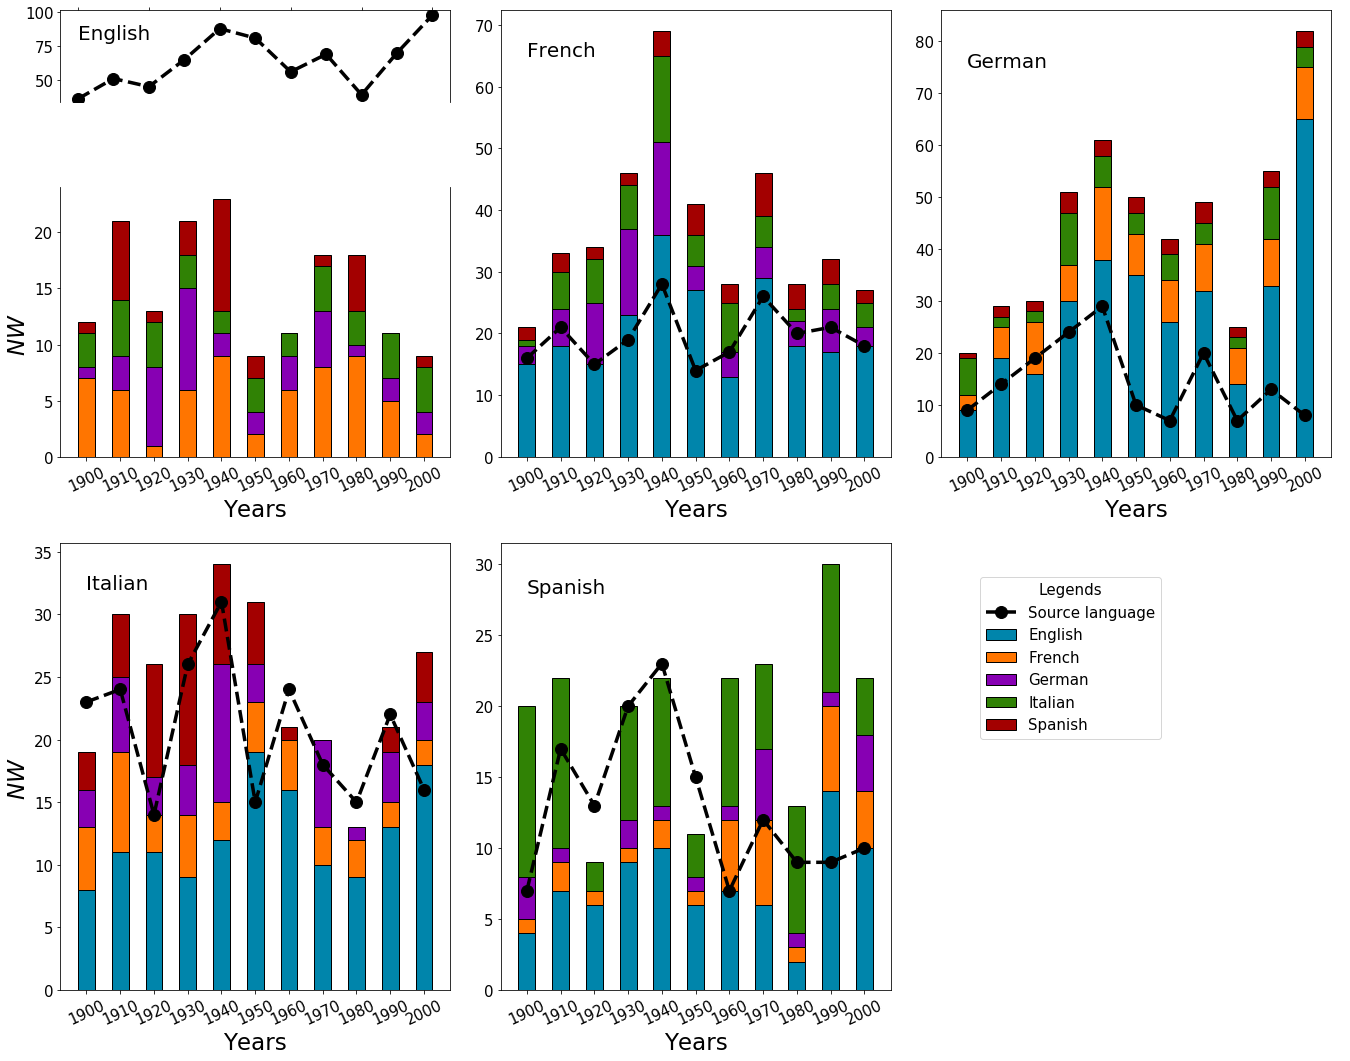
\includegraphics[scale=.35]{NW_A.png}
	\caption{{\bf Number of new migrant words per decade.} 
Number of new migrant word going from one language to the rest (dotted
curve), for each decade of the XX century. The number of 
new migrant words coming to a language is shown as a bar plot, discriminated
by the language that contributes the words. 
Only English has
% been the language that has 
migrated more words than it has received.
Consequently, the largest proportion of migrant words in the other languages
come from English. French, German, Italian and Spanish have received more words
during the second half of the century, after the end of World War II.	
% \cpnote{Explicar la curva punteada, poner los colores aparete, digamos en una
% leyenda como un sexto grafico un poco, y describir mejor y analizar tantito
% (una frase).}
\cpnote{Achicar el espacio en blanco para el plot de ingles. Agrandar al mismo 
tamaño la fuente de las Legends para que sea del tamaño 
de la fuente del idioma en cada plot. Quitar lo que dice ``Legends'', }
% 		\caption{{\bf New migrant words that migrate from one source
% language to the different receiving languages.} Among language such as sources
% (dotted plot) and receivers (bar plot) of new words, only English language has
% been the language that has migrated more words than it has received.
% Consequently, the largest proportion of migrant words in the other languages
% come from English. French, German, Italian and Spanish have received more words
% during the second half of the century, after the end of World War II.	
% \cpnote{Explicar la curva punteada, poner los colores aparete, digamos en una leyenda como un sexto grafico un poco, y describir mejor y analizar tantito (una frase).}
}
\label{fig.NMW_A}
\end{adjustwidth}
\end{figure} % }}}

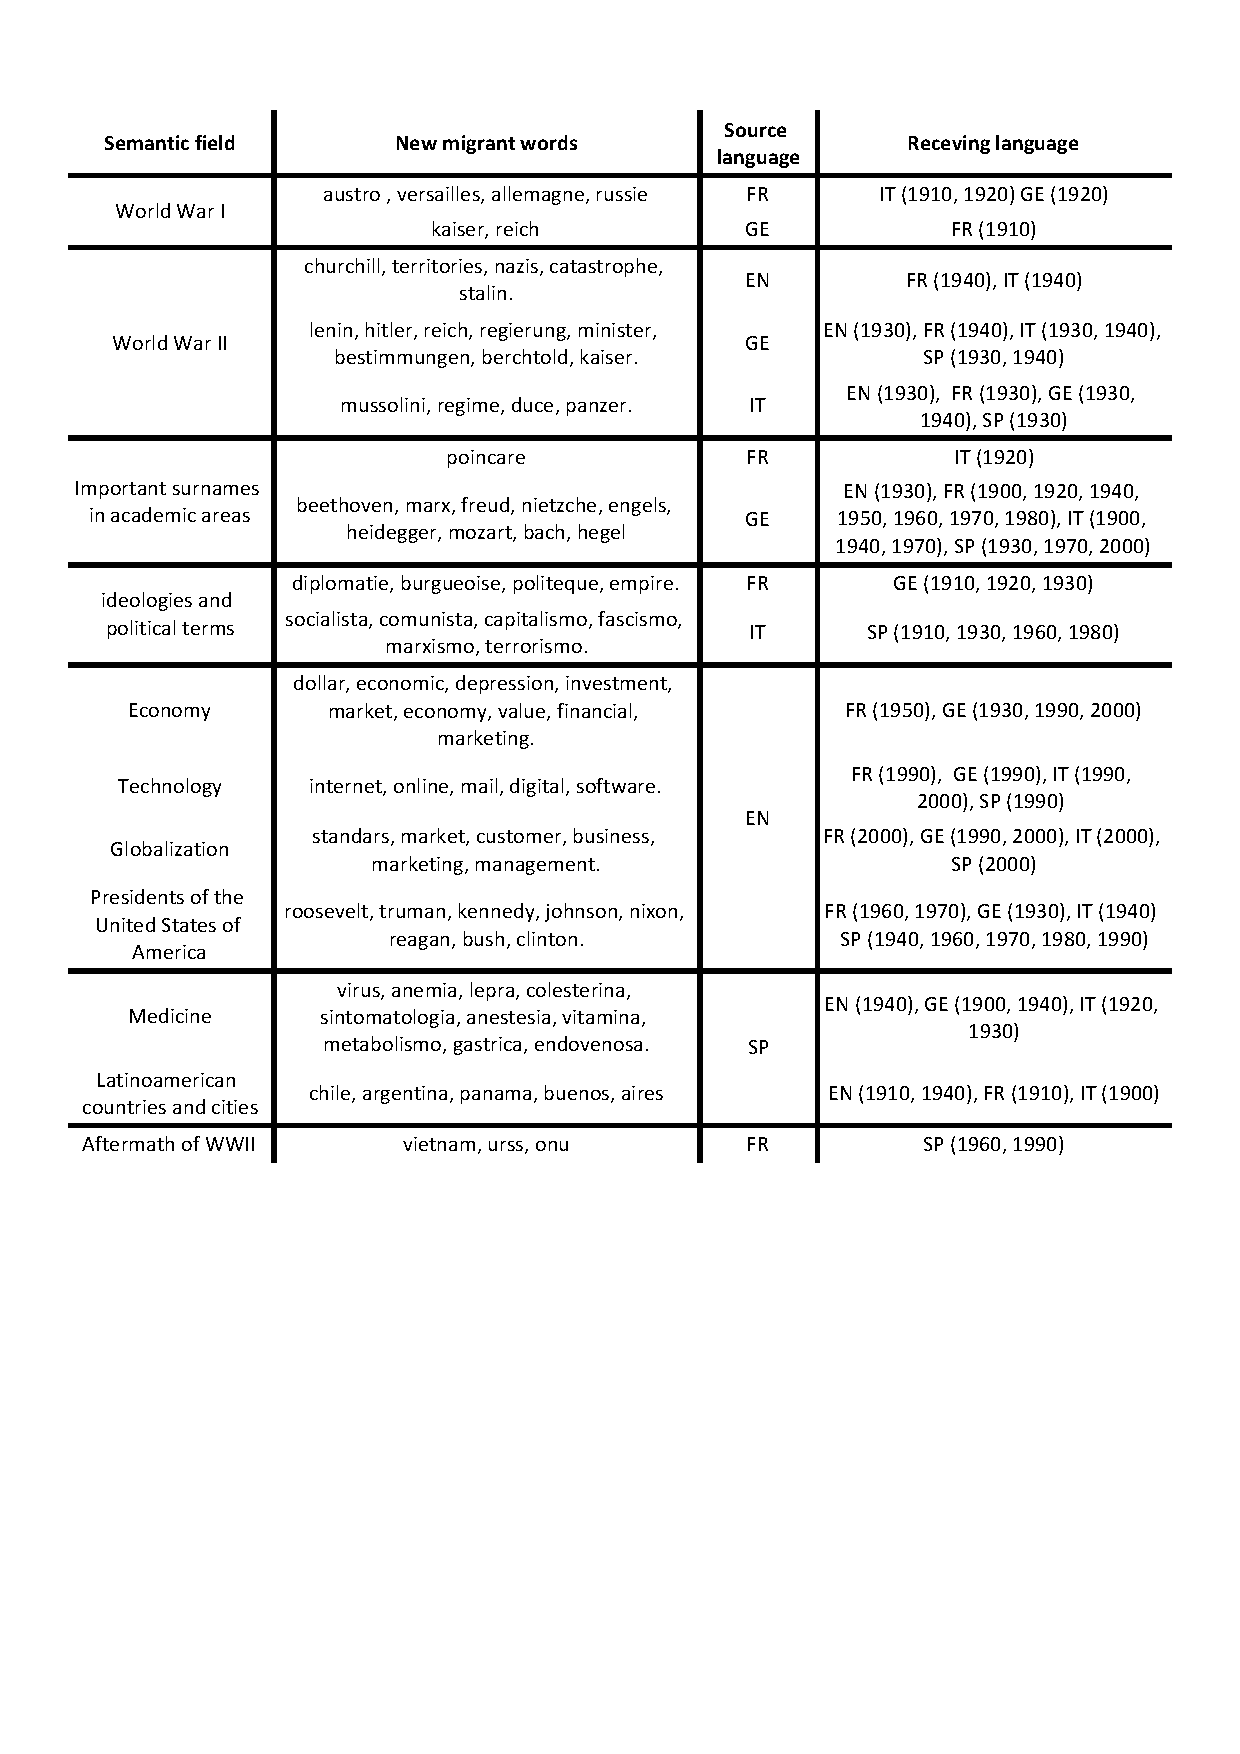
\includepdf[pages=-]{Table_NMW.pdf}

%\begin{figure}[!h]
%	\begin{adjustwidth}{-1.2in}{0in}
%	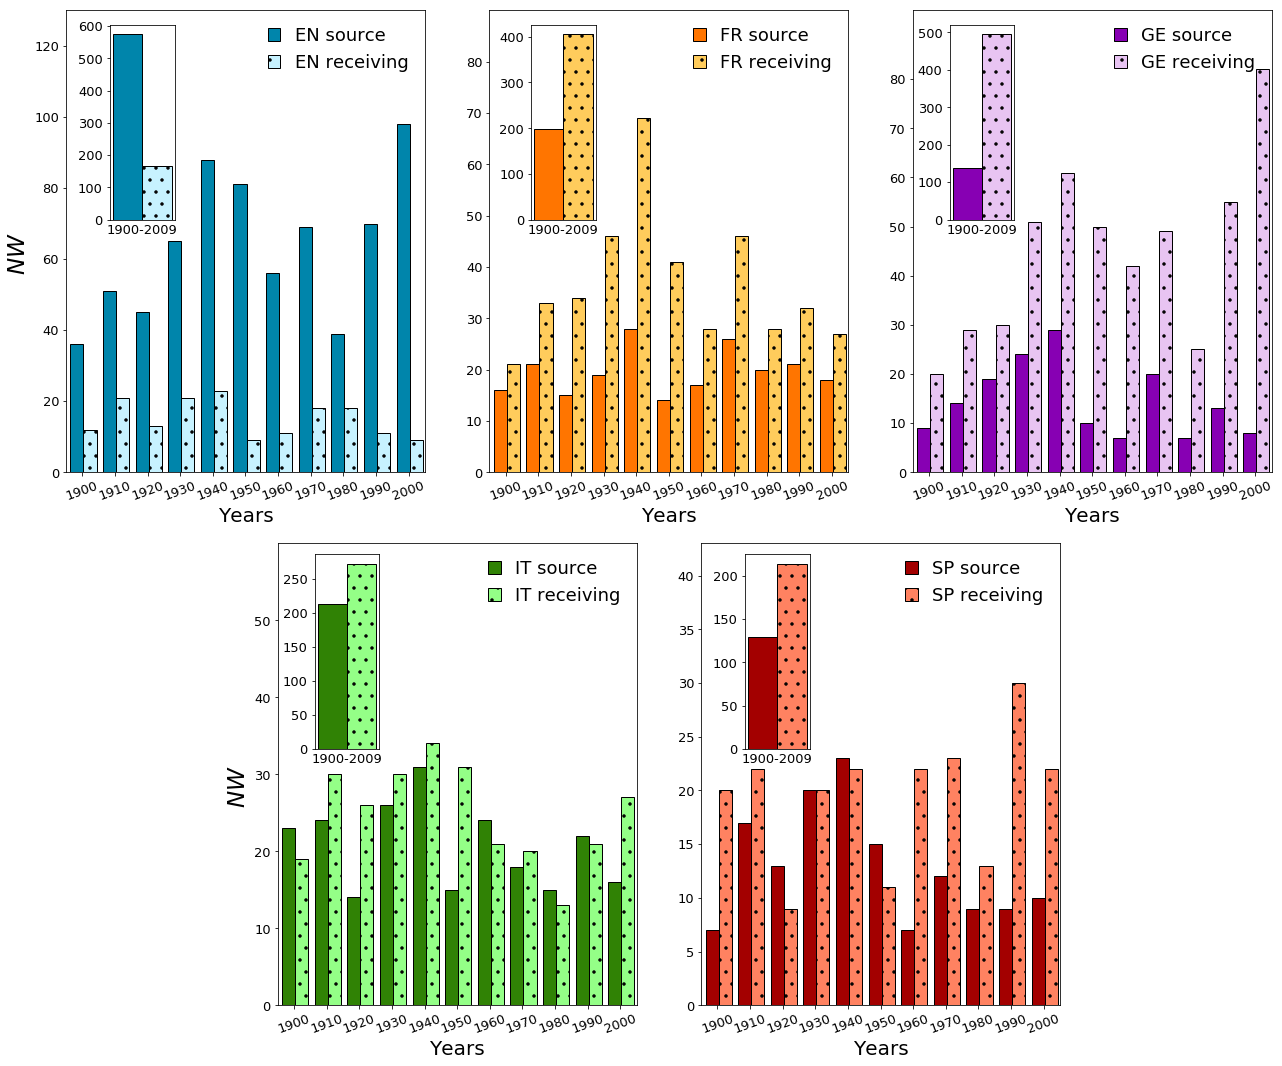
\includegraphics[scale=.35]{NW_OR.png}
%	\caption{{\bf Languages as sources and receivers of new words.} 
%\cpnote{Josué, toca primer describir el grafico y luego analizarlo. Te falta la descripción.}
%During the 20th century, only English language has been the language that has migrated more words than it has received. French, German, Italian and Spanish have received more words during the second half of the century, after the end of World War II.\cgnote{estandarizar ejes $y$???}}
%	\label{fig.NMW_OR}
%	\end{adjustwidth}
%\end{figure}

It is also notable that the French and German languages were mainly
languages influenced by others, since they received more words than
they contributed. This trend is more appreciable since 1940 after the end of
World War II. In addition, since 1980, German has obtained 30 new words every
decade compared to the previous decade, consequently it has been the largest
receiver in the last 30 years.

The Italian language decade by decade, contributes almost the same number of words as those it receives, the only exceptions occurred in the decades of the 1920s and 1950s after the end of the First and Second World War, decades where it was mainly a receiving language. Finally, the Spanish language in 1930 and 1940, also contributed the same number of words as those it received; in the other decades it was primarily a receiving language.

\cpnote{Siento que el parrafo es muy negativo. Cual es el punto central de lo que quieres
decir? Quizá a partir de ahí redisñar el parrafo}
The previous results only manage to show in which decades the languages
contributed or received more words, it being evident that half a century after
the end of World War II, the English language began to be primarily the source
language that contributed the most words to others. 

\cpnote{De nuevo, reingenierpia de parrafo. La primera frase debe tener la idea 
principal, y las siguientes expandiendolas}
Another way to visualize the previous results is shown in Fig~\ref{fig.NMW_A}.
This shows how the new migrant words that each source language contributed are
distributed in the different receivers for each decade \cpnote{Muy complicada
esta frase. Simplifica}. To exhibit that migrant
words are related by their meaning, some new migrant words that were related to
certain semantic fields are display in table~\ref{tab.NMW}; specifying the
language they come from, to which languages they migrated and the decades they
migrated. \cpnote{Esta es una idea interesante, pero como está, interrumpe el análisis
de donde vienen las palabras. Siento que toca justificar o mencionar que esas palabras
vienen agrupadas, y que es conveniente analizar los paquetes. Quizá no veo el flujo del
articulo, tu lo sabras mejor, Josué (acabo de comenzar a reeditar hace dos parrafos}




% % Place tables after the first paragraph in which they are cited.
% \begin{table}[!ht]
% \begin{adjustwidth}{-2.25in}{0in} % Comment out/remove adjustwidth environment if table fits in text column.
% \centering
% \caption{
% {\bf Table }}
% \begin{tabular}{|l+l|l|l|l|l|l|l|}
% \hline
% \multicolumn{4}{|l|}{\bf Heading1} & \multicolumn{4}{|l|}{\bf Heading2}\\ \thickhline
% $cell1 row1$ & cell2 row 1 & cell3 row 1 & cell4 row 1 & cell5 row 1 & cell6 row 1 & cell7 row 1 & cell8 row 1\\ \hline
% $cell1 row2$ & cell2 row 2 & cell3 row 2 & cell4 row 2 & cell5 row 2 & cell6 row 2 & cell7 row 2 & cell8 row 2\\ \hline
% $cell1 row3$ & cell2 row 3 & cell3 row 3 & cell4 row 3 & cell5 row 3 & cell6 row 3 & cell7 row 3 & cell8 row 3\\ \hline
% \end{tabular}
% \begin{flushleft} Comentarios
% \end{flushleft}
% \label{tab.NMW}
% \end{adjustwidth}
% \end{table}

The English language as the source language, contributed more words to the
French, German and Italian languages, between the 1930s and 1950s. In this
period the words found are related to the semantic field of World War II, where
countries such as the United States of America, the United Kingdom, France,
Italy and Germany were involved\cpnote{; the influence of such event can 
be appreciated in table \ref{table:lquesea}}. In the last twenty years (1980-2000), the
French, German, Italian and Spanish languages have received from English words
with content on economics, technology and globalization; we associate this
increase with the fact that the English language has been positioned as the
common language for communication and for spreading information. \cpnote{Sustentar
esta información con una tabla. }

In the case of the French language, its influence as a source language
increased between the 1920s and 1940s, where the main recipient languages were
English, French and Italian. The words that migrated to these languages were
related to both World War I and II, highlighting exonyms from
French to cities, countries and political ideologies that were relevant in such
warlike conflicts. \cpnote{De nuevo, sustentan con tabla}

For German as the source language, the largest number of words migrated to other languages between the 1920s and 1940s. The role of Germany in the warlike conflicts of the 20th century, led to the migrations of the semantic field of war in these decades. Another important semantic field that characterizes words with German words, is the important surnames of German-speaking characters who excelled in certain academic areas, such as psychology, philosophy and music; this field shows an influence of the cultural type not only of the German language, but also of the German-speaking academy.

In Italian, the semantic field that characterizes its migrant words  is again the World War II, showing an increase of the Italian language between 1920 and 1940. In addition to the words of the semantic field of World War II, in Spanish also migrated words related to political ideologies that were relevant in the aftermath of World War II.

%\begin{equation}\label{key}\end{equation} 

The migrant words from Spanish that reached the other receiving languages, those whose content refers to the field of medicine stand out, these words being the ones that originated the greatest contribution of Spanish in the first half of the 20th century. Finally, names of Latin American countries  which suffered from economic crises, were also found.

Among the multiple combinations of source language and recipient language, the most common semantic fields are of a historical nature, highlighting the one referring to the World War II, where words referring to it migrated in all languages.

\cpnote{siento que está un poco repetitivo los párrafos. Que tal organizar por campos 
semánticos y decir que asi es la mayoría de migraciones, y quizá listar las que
se hicieron, y luego irse a los otros casos, como medicina y esas vainaS? Que
opinas, Jouse?}


%In the multiple combinations of source language and recipient language, the most common semantic fields are of a historical nature, highlighting the one referring to the Second World War, where words referring to it migrated in all languages. In addition, it was possible to show that languages have been influential in different areas, English in technology, economics, politics and globalization; French and Italian in war and political ideologies, German in addition to war in academic areas, and Spanish in medicine.
% }}}
% }}}
\section*{Accumulated words} % {{{
% Intro {{{


\cpnote{Dale una iterada a esta intro, porfa. Por lo menos hasta la linea 243}
\jmnote{Rescribi esta seccion,  deje el parrafo 'malo' como referencia}

The previous results show that words travel from one language to another in groups belonging to a common semantic field. Nevertheless, we cannot associate them with a number that interprets how much influence has one language on another.

To obtain such a number, we will focus on migrant words in the years after the first year they migrated, observing how their frequency varies over time. For example, a migrant word will begin to be influential if its frequency increases over time. Since we are dealing with groups of words, we define as accumulated migrant words, those words with source language $A$ that already appeared in a´ receiving language $B$, and for a given year they do so again.

If we take the list of the most used words of $B$ in a year $t$ (the words are ranked according to their frequency), we add the frequencies of the accumulated migrant words of $A$ that have a rank $j$; we normalize the this quantity by dividing it by the frequency of the five thousand words that make up the list.
\begin{equation}
\label{ec.fuso}
\underset{ \text{\tiny A} \to  \text{\tiny B} }{U}(t) = \frac{\sum_{j} f(j)}{\sum_{k=1}^{5000} f(k)}.
%\frac{ \underset{ \text{\tiny A} \to  \text{\tiny B} }{P}(t)}{\underset{\text{\tiny B}}{F}(t) }.
\end{equation}

We define this new value as the \textbf{Use} $\underset{ \text{\tiny A} \to \text{\tiny B} }{U}(t)$ of $A$ in $B$ , and it is the measure that quantifies the influence. It will then be said that the influence of $A$ has increased on $B$, if in an interval of time $\Delta t$ the use of $A$ on $B$ increases. Finally, to quantify the change in use within a time interval, the term ratio of words per year (wpy) will be used, obtained by dividing $\Delta U$  by  $\Delta t$.


\noindent\rule{10cm}{0.4pt}

The previous results of classifying migrant words according to a semantic
field, shows which areas have been influential for there to be a movement of
words among languages\cpnote{Mas bien algo como 
The previous results show that words travel from one language to another in groups
belonging to a common semantic field.}. Nevertheless, there is still no answer neither on which
language has been more influential over another, nor how the influence
occurred\cpnote{A que te refieres con eso ultimo de ``how the influence occurred''}.

\cpnote{Comenzar por una motiviación o necesidad de la definición. Algo mas suave.}
We define as accumulated migrant words those words with source language $A$
that had already appeared in a receiving language $B$, and for a given year
they do so again\cpnote{Demasiado choro. Al grano mejor.}. The difference between the new migrant words and the
accumulated migrant words, is that they will only be new in the first year of
appearance, later on they will become accumulated.

With the accumulated migrant words, we construct a function to quantify the
influence of one language on 
another. The procedure to
achieve such quantity begins with taking from a year $t$ the list of the five
thousand most used words of the recipient language $B$\cpnote{Demasiado choro. Al grano mejor.}. Once this is done, we
add the frequency $f(k)$ of the five thousand most used words of the receiving
language $B$ in year $t$, where $k$ is the rank of each word
\begin{equation}
\label{ec.ftot}
%\underset{\text{\tiny B}}{F}(t) = 
\sum_{k=1}^{5000} f(k).
\end{equation}

Later in the list of words, we distinguish and add the frequency $f(j)$  of
those with rank $j$ that are accumulated migrants and that come from the source
language $A$ \cpnote{No entiendo para nada esta frase. Ni como se distinge de
la anterior.}
\begin{equation}
\label{ec.fpres}
%P^{y}_{\text{A} \to \text{B}} = \sum_{j} f(j)
%\underset{ \text{\tiny A} \to  \text{\tiny B} }{P}(t) = 
\sum_{j} f(j).
\end{equation}

It is called as the \textbf{Use} $\underset{ \text{\tiny A} \to \text{\tiny B} }{U}(t)$ of $A$ in $B$ to the result of normalizing the previous quantity after dividing it by the frequency of the five thousand most used words, given by \ref{ec.ftot}.

\begin{equation}
\label{ec.fuso1}
\underset{ \text{\tiny A} \to  \text{\tiny B} }{U}(t) = \frac{\sum_{j} f(j)}{\sum_{k=1}^{5000} f(k)}.
%\frac{ \underset{ \text{\tiny A} \to  \text{\tiny B} }{P}(t)}{\underset{\text{\tiny B}}{F}(t) }.
\end{equation}
This new quantity is the one that will quantify the influence of $A$ on $B$. It will be said that language $A$ has influenced language $B$ more if within a time interval $\Delta t$, the use of $A$ in $B$ increases; this will mean that the accumulated words have increased their frequency.

Finally, to quantify the change in use  $\Delta U$ within a time interval $\Delta t$, the term ratio of words per year (wpy) will be used, obtained by dividing $\Delta U$ by $\Delta t$.
% }}}
\noindent\rule{10cm}{0.4pt}


\subsection*{The use among languages} % {{{
\cpnote{De nuevo, hay solo una subseccion. Ver que hongo}

We obtained with the previous method, the accumulated migrant words among all the possible combinations from a source language to a receiving language, in the 269 years (1740-2009) of the dataset. Then in each combination we applied the equation~\ref{ec.fuso} to realize the use in the years between 1900 and 2009. To simplify the reading we establish s set of abbreviations to distinguish the languages, EN for English, FR for French, GE for German, IT for the Italian and SP for Spanish. In addition, to name some combination of source  and receiving languages, two abbreviations will be used, the first being the source language of the accumulated migrant words, and the second the receiving language of them, for example EN-GE, means the migrant words from English that are present in the German.

The migrant accumulated words between pairs of language were ordered by the year in which they appeared and in descending order in their frequency, therefore the first place in the ranking is occupied by the most frequent word in that year, the second for the second most frequent, and so on.

The Fig~\ref{fig.UT_art} shows the use of a source language, in all receiving languages, as the use in each case may have a different scale, the data were normalized by dividing them by their average value, this with the intention of observing in which time interval the use was more affected (increase or decrease more than in the others), since this will indicate that accumulated words were more or less influential. 


\begin{figure}[!h]
	\begin{adjustwidth}{-6cm}{1cm}
		\centering
		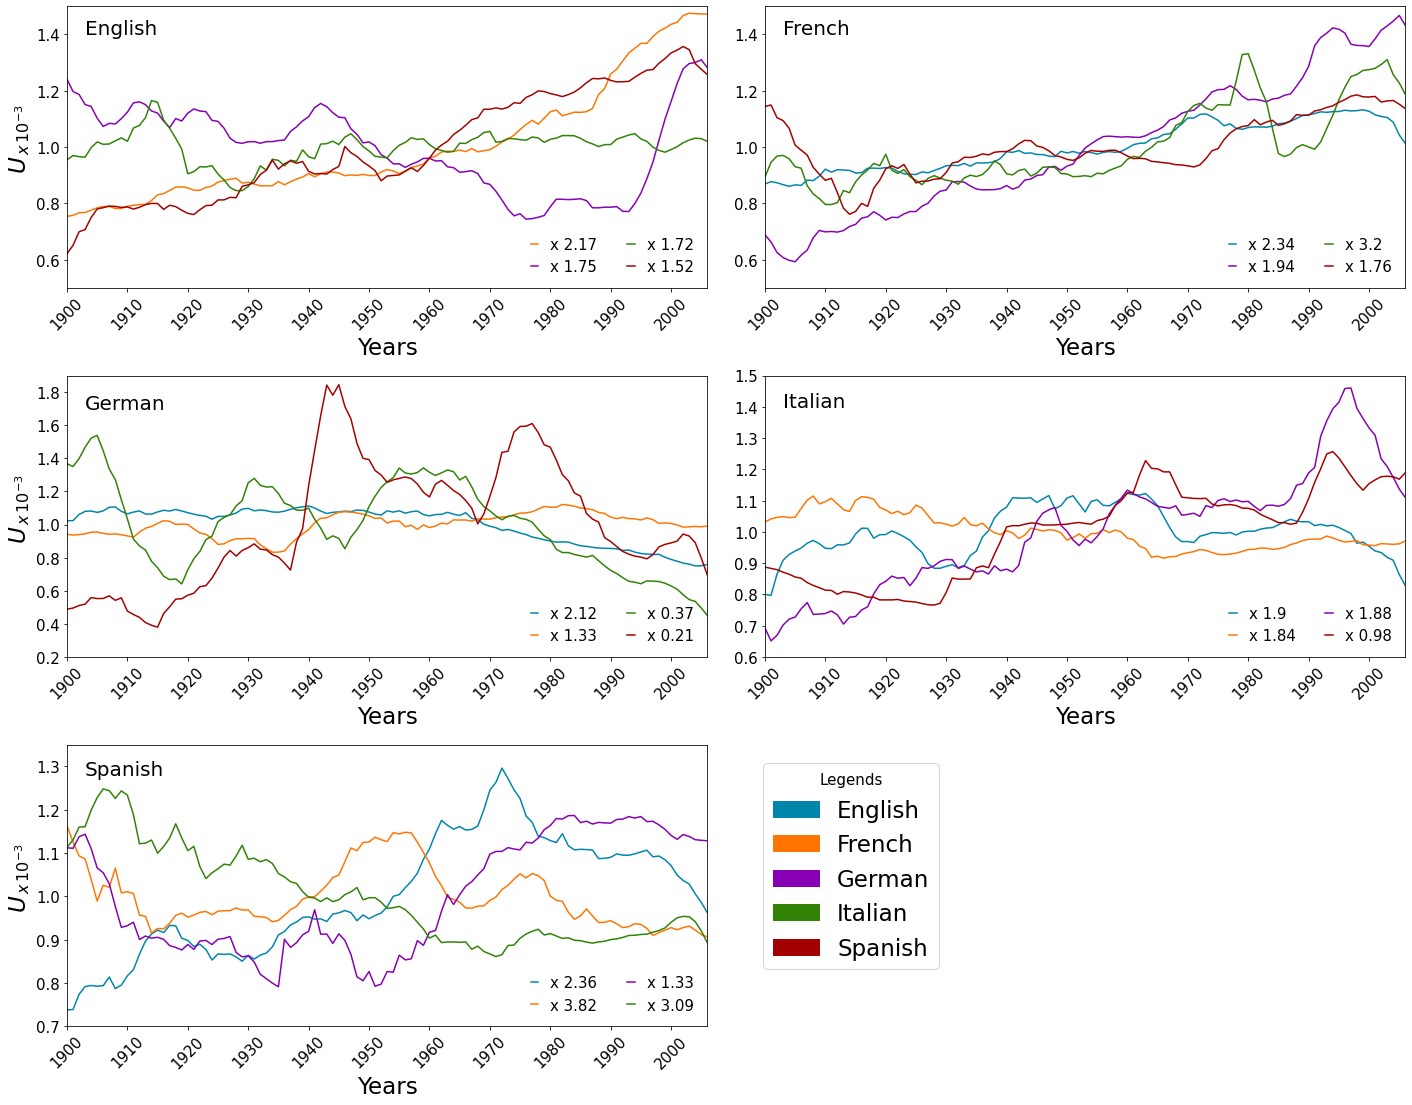
\includegraphics[scale=0.38]{USO_A.png}
		\caption{{\bf The Use among languages.} All language pairs.....}
		\label{fig.UT_art}
	\end{adjustwidth}
\end{figure}
% }}}
\subsubsection*{English} % {{{

The use of English in French, Italian and Spanish began to increase after 1930, while in German it was until 1990. We associate the cause of these increases with the emergence of the United States as a world power, after finishing the WWII and  impose its economic model as well as the development of science and technology. The accumulated migrant words that are present in all receiving  languages are \textit{capital}, \textit{dollar}, \textit{invesment}, \textit{relations}, \textit{market}, \textit{company}, \textit{development}, \textit{financial},  \textit{institutions}, \textit{internet}, \textit{windows} and \textit{software}. Those can again be associated with semantic fields such as economics, technology, and globalization.

% }}}
\subsubsection*{French} % {{{

The increase in the influence of French in the other languages occurred in English between 1920 and 1970, in German between 1900 and 2009, and in Spanish between 1970 and 1995. In these years the words that increased its frequency are from the semantic fields of religion such as \textit{dieu} , \textit{évêque}, \textit{dime}, \textit{religion}, \textit{saint} and \textit{église} (iglesia); while \textit{reine}, \textit{forteresse}, \textit{napoleon}, \textit{guerre}, \textit{imperiale}, \textit{bastille}, \textit{royal} and \textit{bourgeois} are from French Revolution.

In Italian between 1950 and 1970, in addition to the above words,\textit{raisins}, \textit{vin}, \textit{vignoble} y \textit{recolte} were found, the common meaning of which is the wine industry, a common industry in France and Italy.

% }}}
\subsubsection*{German} % {{{

Spanish between 1935 and 1940 was the language where German had the greatest increase among all receiving languages; followed by the French between 1930 and 1945; in both  the words that are present are the surnames of German-speaking characters who excelled in academic areas, such as \textit{marx}, \textit{Freud}, \textit{heidegger}, \textit{nietzsche}, \textit{hegel}, \textit{engels} and \textit{mozart}.

In English and Italian, the biggest change was between 1960 and 2009, where the use of German decreased. In this period the words that lost influence are referred to the World War II, among them \textit{berlin}, \textit{marx}, \textit{hitler}, \textit{lenin}, \textit{testen}  and \textit{reich}.
% }}}
\subsubsection*{Italian} % {{{
 
 
The influence of Italian came mainly from two semantic fields, the WWII 
with \textit{mussolini}, \textit{fascismo}, \textit{battaglia}, \textit{regime}, \textit{sociale} and \textit{liberale}; and the religion with \textit{santo}, \textit{suora} (monja) and \textit{cattedrale}. These semantic fields are responsbale for the increase in English between 19630 and 1940, in German between 1950 and 1995, and in Spanish between 1930 and 1960.
 
In French, Italian has the lowest influence, where the aforementioned words began to be less frequent between 1940 and 1960.
% }}}
\subsubsection*{Spanish} % {{{

The influence of Spanish in English between 1920 and 1970, was due tu historical and cultural facts, since countries in Latin American as  \textit{mexico}, \textit{panama}, \textit{chile}, \textit{cuba}, \textit{peru}, \textit{colombia}, \textit{argentina} and its capital \textit{buenos} \textit{aires};  and states in the United States  where a large part of the Spanish-speaking population is concentrated as \textit{california} and \textit{florida}, were increased their frequency.

In German after WWII, and in French between 1930 and 1955, the mainly words involved in that increse are, \textit{terapia}, \textit{anemia}, \textit{lepra}, \textit{tumor}, \textit{syphilis}, \textit{virus} and \textit{renal}.

% }}}
% }}}
\section*{Rank diversity} % {{{

\cpnote{Why are we interested in rank diversity that has not been understood in the 
previous sections?}
Since the accumulated migrant words are organized by year, and at the same time
in each year the words are ordered in ascending order in rank, then over time,
the same rank can be occupied by different words. One way to quantify how many
different elements can occupy the same rank within the same corpus is through
rank diversity $d(k)$ \cpnote{this last sentence belongs to a paragraph introducing rank
diversity. I think that we must start saying the idea that we want to quantify. That, 
in a paragraph. Then another paragraph that really introduces the measure, which I think
is still laking. Maybe a single paragraph that contains both ideas.}.

Rank diversity has been used in datasets of the most used words in six
Indo-European languages, and in sports and game classifications. Although in
each case the criteria for establishing a ranking are different, in both there
is a common result: for the same set of data that have had different rankings
over time, it is true that the lowest ranks are always occupied by fewer
elements, thereby as the range increases, the number of elements that occupy it
also does them.

After applying the rank diversity in each source language and receiving language pair, the diversity values resemble a logarithmic curve, as can be seen in Fig~\ref{fig.DR_art}. We proposed the curve $d(k) =  \alpha \ln(k) + \beta.$ to fit the rank diversity where the parameters $\alpha$ and $\beta$ were obtained with a linear regression. With the corresponding linear regression of each language pair, the reliability of the fit with the coefficient of determination $R^{2}$ was verified. If $ a_ {k} $ represents the value of the adjustment equation when evaluating it in the range $ k $, $ d_ {k} $ is the diversity obtained for the same range and $ \ bar {d} $ is the average of all values of the diversity, then $R^{2}$ is expressed as:
\begin{equation}
R^{2} = 1 - \sum_{k = 1} \frac{ \left( \,d_{k} - a_{k} \,\right)^{2}  }{ \left( \, d_{k} - \bar{d} \,\right)^{2} }.	
\label{ec.r2_diversidad}
\end{equation}

\begin{figure}[!h]
	\begin{adjustwidth}{-2.5cm}{1cm}
		\centering
		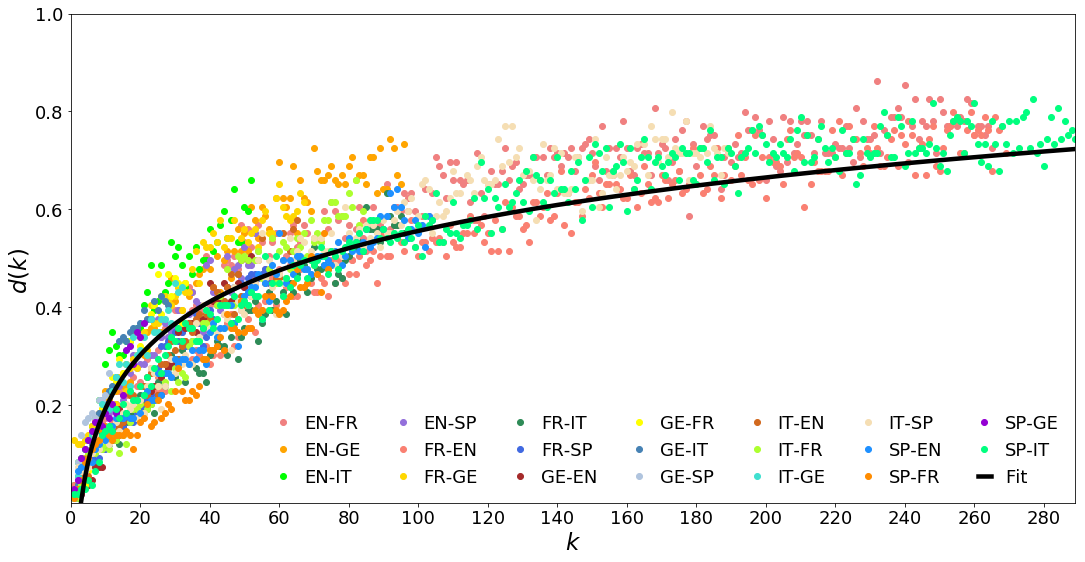
\includegraphics[scale=.38]{DR_art.png}
		\caption{{\bf Rank diversity of accumulated migrant words among languages.} All language pairs show a logarithmic behavior regardless of the number of ranks where the rank diversity was applied. The reliability of the fit to a logarithmic curve of the 20 combinations is on average $R^{2}= 0.88 \pm 0.04$.\cgnote{hacer eje $x$ log}}
		\label{fig.DR_art}
	\end{adjustwidth}
\end{figure}


Fig~\ref{fig.DR_art} also shows the graph of equation $d(k) = 0.16\ln(k) - 0.17$, obtained after averaging the coefficients $\alpha$ and $beta$ for each language pair. It is observed that the behavior of diversity increases as the rank also increases, regardless of whether the corpus has few or many ranks (14 in German-Spanish, 290 in Spanish-Italian). With this, it can be concluded that, the migrant accumulated words in the middle and high ranks are the ones that tend to change their position the most within a ranking over time.


%PLOS does not support heading levels beyond the 3rd (no 4th level headings).

% }}}
\section*{Robustness} % {{{

The method of the use of one language in another, showed that the words of certain semantic fields decrease their rank if the use tends to increase. Nevertheless, the inverse case cannot be concluded, that is, we do not know if the use of a language increases as a consequence of a group of words decreasing its rank, nor do we know how stable is the use among languages if certain words were not taken; since within the accumulated words of one language in another, only a few belong to a specific semantic field.

To check the stability of the use among languages and the importance of omitting certain elements, we constructed a method to interpret the robustness of the corpus. This consisted of taking the original set (the one obtained in the previous section) of the accumulated words of a pair of source language and receiving language, and of this, eliminating a certain group of words, in order to obtain a reduced set; in both,  equation~\ref{ec.fuso} is used to obtain the use between the years 1900 and 2009.

The next thing is to determine how similar the use of both sets are, we normalized the values of both sets, after dividing them by the average value of each one; then for each year $t$ we obtain the distance between each value of original use $u_{t}$ and its corresponding value in reduced use $r_{t}$; the average of them gets the \textbf{average distance} $\left\langle D \right\rangle$, which will be the one that quantifies the similarity of the results, indicating a greater similarity if it is close to zero.

%We defined as the \textbf{conversion factor} $F_{c}$ as the result of dividing the average of the reduced use by the average of the original use. After normalization, for each year $t$, we obtain the distance between each value of original use $u_{t}$ and its corresponding value in reduced use $r_{t}$; the average of them gets the \textbf{average distance} $\left\langle D \right\rangle$, which will be the one that quantifies the similarity of the results, indicating a greater similarity if it is close to zero.
\begin{equation}
\left\langle D \right\rangle  = \frac{1}{N}\sum_{t=1}^{N} \left| u_{t} - r_{t} \right|  .
\label{ec.Davg}
\end{equation}

\subsection*{Elimination characteristics}

To answer how stable the sets are if we altering them, we first verify that in each year the accumulated migrant wors between two languages, obey Zipf's law $f~1/k$ if they are order ascending by their rank Fig~\ref{fig.ZL_receiving}; from this it is understandable to deduce that the use between languages would be more affected if the words with the lowest ranks are eliminated, since the sum of the frequencies of this group is greater than the sum of the frequencies of the words with the highest ranks.

\begin{figure}[!h]
	\begin{adjustwidth}{-2.5cm}{1cm}
		\centering
		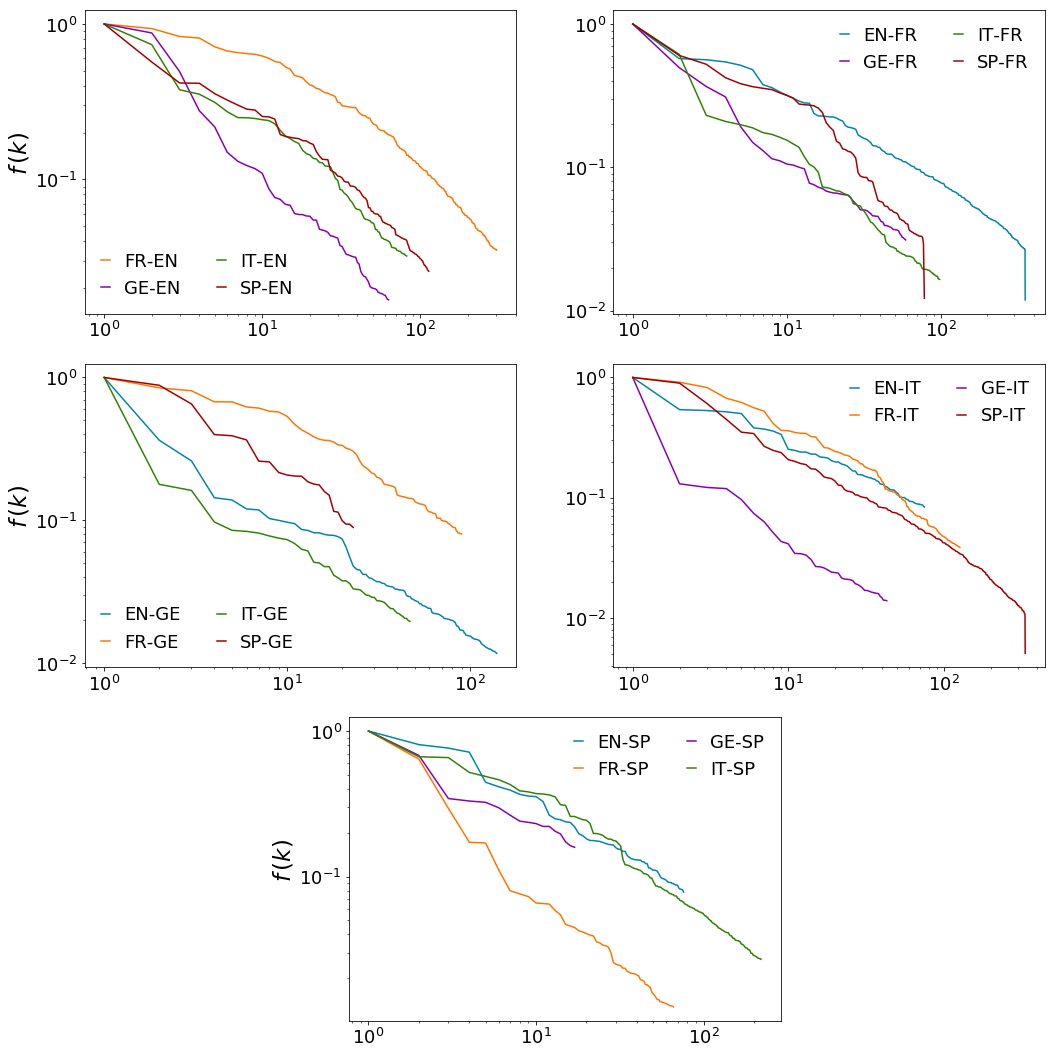
\includegraphics[scale=.38]{ZL_receptor.png}
		\caption{{\bf Zipf's law of the accumulated migrant words, grouped by receiving language.\cgnote{m\'as que Zipf's law, distribuci\'on de frecuencias, se podr\'ia hacer ajuste con Zipf e indicar exponente.}} }
		\label{fig.ZL_receiving}
	\end{adjustwidth}
\end{figure}


Another way to tell the previous deduction, is thinking that if the sum of frequencies is the same in two sets, where the first is made up of words with low ranks, and the second by words with high ranks, the second set would have to have more items than the first. With these ideas, in each source language and receiving language pair, we carry out two types of elimination, in the first we begin to eliminate the words with the lowest ranks and little by little increasing the portion of words eliminated $R_{p}$ (from 1$\%$ to a 99$\%$) until the words with the highest ranks are
were covered Fig~\ref{fig.RP_low}; the second way was the opposite case, beginning to eliminate a small portion of those worsd with highest ranks and gradually increasing it until cover the lower ranks Fig~\ref{fig.RP_high}. In both cases, each time the eliminated portion was increased, the average difference was calculated to observe the similarity.


\begin{figure}[!h]
	\begin{adjustwidth}{-2.5cm}{1cm}
		\centering
		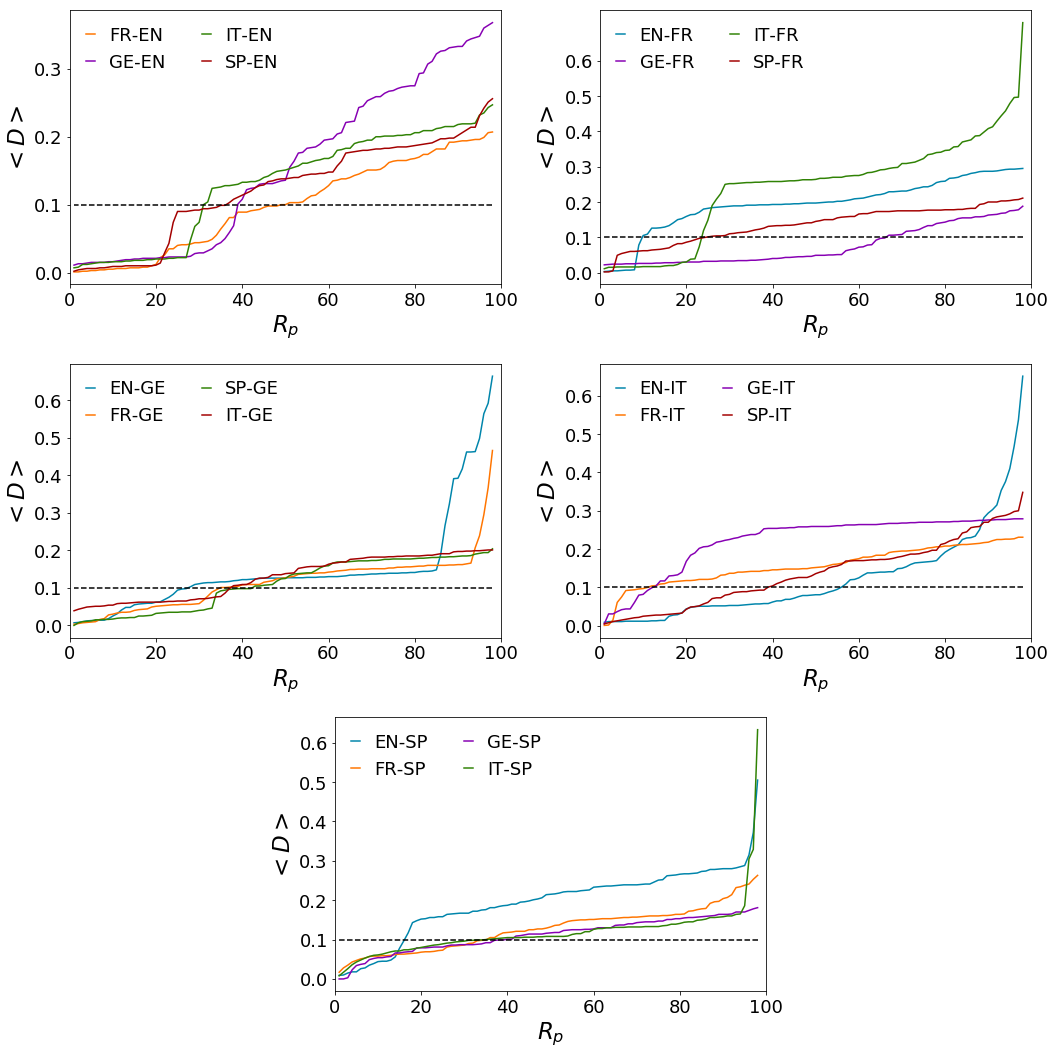
\includegraphics[scale=.38]{Rp_bajos.png}
		\caption{{\bf Portion of eliminated words with lows ranks.} }
		\label{fig.RP_low}
	\end{adjustwidth}
\end{figure}


\begin{figure}[!h]
	\begin{adjustwidth}{-2.5cm}{1cm}
		\centering
		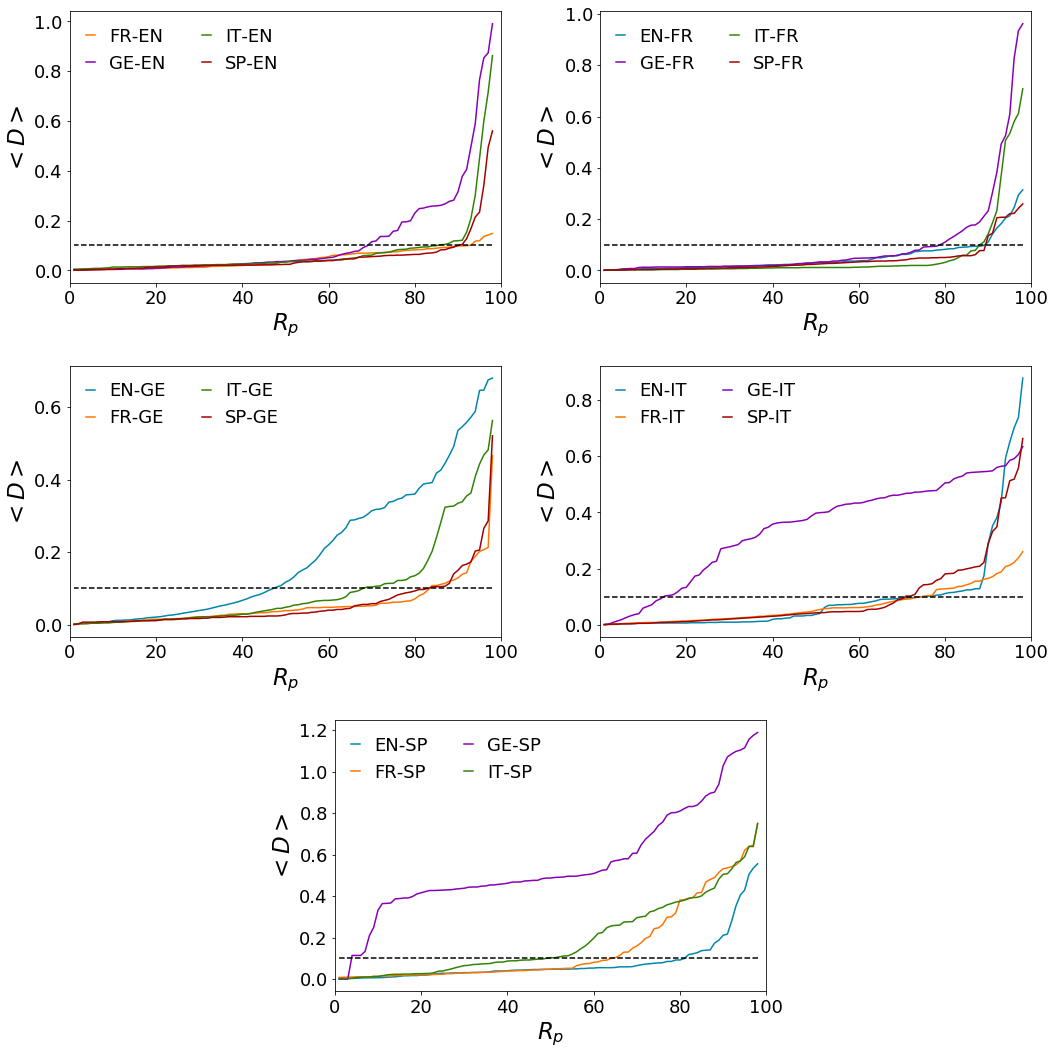
\includegraphics[scale=.38]{Rp_altos.png}
		\caption{{\bf Portion of eliminated words with high ranks.} }
		\label{fig.RP_high}
	\end{adjustwidth}
\end{figure}

After observing both figures, it is appropriate to say that for the similarity of the use between languages are altered, a greater number of words with high ranks are needed than words with low ranks, in terms of robustness, the sets are more stable if altering them are eliminated those words with the highest ranks, that is, those with the lowest frequencies.

This result, despite showing the stability of the sets when eliminating words from them, can be counterproductive with the results of the previous sections, since in those we try to find relationships based on the meaning of the words, and in case of an elimination such relationships would be lost if the words involved have high ranks.

%just multiply the original use by the conversion factor to obtain the reduced use. 

% }}}
\section*{Supporting information} % {{{
% }}}
\section*{Acknowledgments} % {{{

\nolinenumbers

Support by projects CONACyT 285754 and UNAM-PAPIIT IG101421 is acknowledged. 
% }}}
% \bibliographystyle{plos2015}
\bibliography{referencias} 
\end{document}

